\documentclass[12pt]{article}
\usepackage[english]{babel}
\usepackage[utf8x]{inputenc}
\usepackage{amsmath}
\usepackage{tikz}
\usetikzlibrary{arrows,automata}
\begin{document}

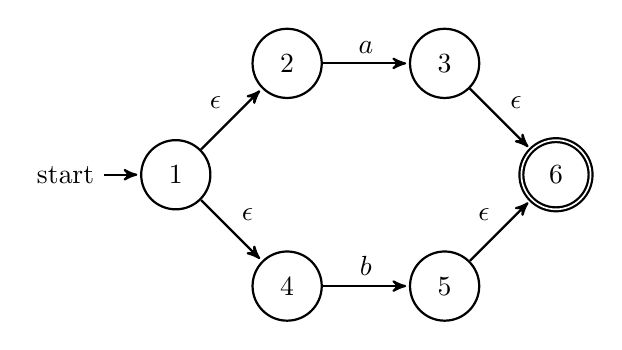
\begin{tikzpicture}[->,>=stealth',shorten >=1pt,auto,node distance=2cm,
    thick,base node/.style={circle,draw,minimum size=8pt}, real node/.style={double,circle,draw,minimum size=17pt}]

  \node[state,initial] (start) {$1$};
  \node[state] (a) [above right of=start] {$2$};
  \node[state] (b) [right of=a] {$3$};
  \node[state] (c) [below right of=start] {$4$};
  \node[state] (d) [right of=c] {$5$};
  \node[state,accepting] (e) [below right of=b] {$6$};
  
  \path (start) edge       node {$\epsilon$} (a)
        (start) edge       node {$\epsilon$} (c)
        (a) edge           node {$a$} (b)
        (b) edge       node {$\epsilon$} (e)
        (c) edge          node {$b$} (d)
        (d) edge       node {$\epsilon$} (e)
         ;

\end{tikzpicture}
\end{document}